\documentclass[10pt,a4paper]{article}
\usepackage[margin=22mm]{geometry}
\usepackage[T1]{fontenc}
\usepackage{lmodern,microtype,graphicx,booktabs,array,caption,xcolor,hyperref,placeins}
\definecolor{ink}{HTML}{253547}
\hypersetup{colorlinks=true,linkcolor=ink,urlcolor=ink}
\captionsetup{font=small,labelfont=bf}
\setlength{\parindent}{0pt}
\setlength{\parskip}{5pt}
\setlength{\tabcolsep}{5pt}
\title{\vspace{-15mm}\textbf{Efficient VLA-JEPA for Robotic Manipulation}\\[3pt]\large CSI 5341: efficiency evaluation}
\author{Noah Sprenger \qquad Fernando Nogueira}
\date{2026-10-02}
\begin{document}
\maketitle
\vspace{-7mm}
\begin{abstract}
We study whether reduced-precision inference and a smaller vision--language backbone lower VLA-JEPA's deployment cost while retaining manipulation success. We compare a pretrained BF16 policy, two decoder-quantized variants, and a SmolVLM2-500M variant requiring reduced fine-tuning. The protocol combines matched LIBERO-Spatial trials, inference measurements, and a training-budget study. The completed protocol evaluates 500 reserved trials per configuration. Success rates are B16 95.0\%, Q8 94.8\%, Q4 95.8\%, S500 2.2\%. Efficiency and paired uncertainty estimates characterize the resulting deployment trade-offs.
\end{abstract}

\section{Study design}
The baseline is \texttt{lerobot/VLA-JEPA-LIBERO}~\cite{vla}. Q8 and Q4 quantize its trained Qwen language-decoder linear layers using LLM.int8~\cite{int8} (outlier threshold 6) and NF4 with double quantization~\cite{nf4}, respectively; the vision tower, embeddings, action head, and world model remain BF16. Quantization happens \emph{after} policy checkpoint restoration. S500 replaces the backbone with SmolVLM2-500M-Video-Instruct~\cite{smol} and projects its decoder representation into the existing conditioning interface. The adaptation recipe freezes SmolVLM and the V-JEPA~2 encoder~\cite{jepa}, training the adapter and compatible action/world predictors. Qwen is evaluation-only. The optional discovery confirmation is reported separately below.

\begin{figure}[ht]
\centering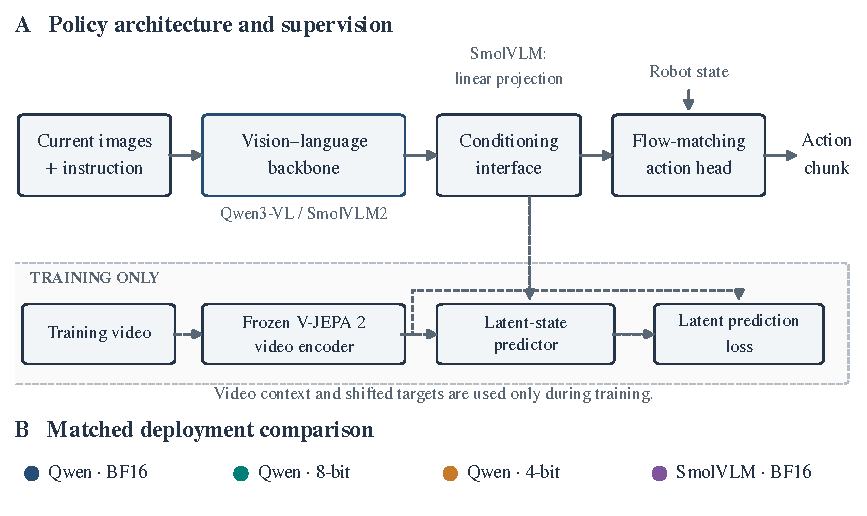
\includegraphics[width=\linewidth]{figures/architecture.pdf}
\caption{Architecture and comparison arms. Solid arrows denote the inference path; dashed connections denote training supervision. The action head also receives robot state. The schematic omits the action-training loss for clarity. All configurations use identical observation/action settings and world-model loading policy.}
\end{figure}

\section{Evaluation methodology}
\textbf{E1: manipulation.} We use all ten LIBERO-Spatial tasks~\cite{libero}, batch size one, matched initial states and per-episode random seeds. Development uses ten original initial-state vectors per task, excluded by exact hash from the official pruned states. Final evaluation uses all fifty official pruned states per task: 500 trials per configuration. The committed manifest records state-file and state-vector hashes. Development scores are diagnostic and are not pooled with final benchmark scores.

We estimate task-macro-average success and task-level rates with 95\% intervals and task-stratified paired bootstrap differences from B16. Intervals describe uncertainty on this fixed task suite, not generalization to unseen tasks. System failures remain separate from valid unsuccessful robot trials. Final trials do not enter checkpoint selection.

\textbf{E2: efficiency.} On one GPU (NVIDIA GeForce RTX 3090), we time a fixed observation/instruction bank with twenty warm-up predictions and 500 measured action-chunk predictions per repetition (three repetitions). CUDA synchronization brackets each measurement. Outcomes are median/p95 neural-only and observation-to-action latency, peak allocated/reserved GPU memory, parameter count, and serialized weight size. Timings exclude simulator execution and buffered-action retrieval; neural-only timing additionally excludes tokenization and image preprocessing. Memory reduction is not assumed to imply a speedup.

\textbf{E3: adaptation.} We split demonstrations by whole trajectories, reserving 10\% for validation. The completed 500-step pilot established execution feasibility and resource cost. The frozen budget is 10,000 optimizer steps (seed 42), with selection checkpoints at 1,500, 5,000, and 10,000 steps from one continuing run. Selection minimizes sample-weighted held-out total loss; ties favor fewer steps. The pilot projects approximately ten GPU-hours including validation and checkpoint overhead. We use one training seed, so training-seed uncertainty is not estimated. The published baseline and S500 have different training histories; their comparison concerns practical deployment under limited adaptation, not the isolated causal effect of backbone size.

\section{Progress and results}
The frozen local dataset split contains 384 training and 48 held-out trajectories (47,043 and 5,927 frames). Hold out the last ten percent of trajectories per task, rounding up. For checkpoint selection, evaluate twenty evenly spaced held-out frames per task with fixed flow-noise seeds and sample-weighted mean loss. Preserve the published baseline normalization statistics across all arms.
\begin{table}[ht]
\centering\small
\begin{tabular}{@{}lllll@{}}
\toprule
Variant & Success [95\% CI] (\%) & Median / p95 (ms) & VRAM (GiB) & Weights (GiB) \\
\midrule
B16 & 95.0 [92.7, 96.6] & 79.1 / 84.3 & 5.22 & 5.15 \\
Q8 & 94.8 [92.5, 96.4] & 157.4 / 161.4 & 4.00 & 3.84 \\
Q4 & 95.8 [93.7, 97.2] & 93.6 / 97.9 & 3.29 & 3.20 \\
S500 & 2.2 [1.2, 3.9] & 1269.7 / 1277.8 & 3.07 & 2.14 \\
\bottomrule
\end{tabular}
\caption{T1: final matched measurements. Success values use the reserved final initial states; trial counts are recorded in the accompanying results. Latency includes outer observation preparation and action postprocessing; VRAM is peak framework allocation. Weight size uses a consistent safetensors encoding with shared tensors deduplicated. Missing results remain pending. No adaptation is applied to B16/Q8/Q4 in this study. S500 measurements use the checkpoint at step 10,000.}
\end{table}



The frozen adaptation budget is complete. Held-out loss selected step 10,000 (loss 0.254); simulator scores were not used for selection.

\textbf{Measured results.} Q8: 23.3\% lower peak allocated memory, 1.99$\times$ baseline latency; Q4: 36.9\% lower peak allocated memory, 1.18$\times$ baseline latency; S500: 41.1\% lower peak allocated memory, 16.04$\times$ baseline latency. These are deployment measurements on one GPU. Neural-only median/p95 latencies (ms) are B16 71.7/75.6, Q8 152.0/161.4, Q4 85.9/90.1, S500 234.5/235.4. Each neural path first reproduced native outputs on all 100 bank observations under identical flow-noise seeds. Final paired success differences from B16 (percentage points; 95\% bootstrap intervals) are Q8 -0.2 [-1.2, +0.8]; Q4 +0.8 [-0.6, +2.2]; S500 -92.8 [-94.8, -90.6].

\begin{figure}[ht]\centering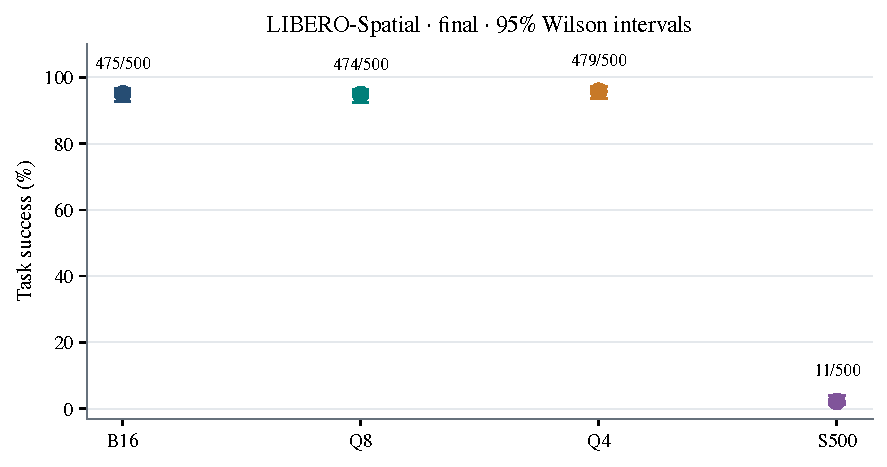
\includegraphics[width=\linewidth]{figures/F1_success.pdf}\caption{Manipulation success on the recorded rollout phase; intervals describe the fixed task suite.}\end{figure}
\begin{figure}[ht]\centering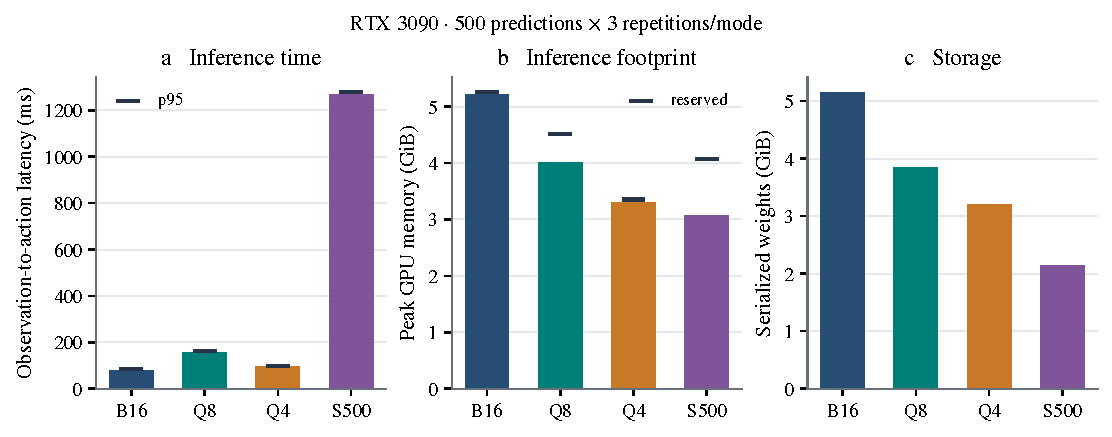
\includegraphics[width=\linewidth]{figures/F2_resources.pdf}\caption{Measured deployment resources on the RTX 3090. Bars show median full observation-to-action latency, peak allocated memory, and safetensors weight size; ticks show p95 latency and peak reserved memory. Batch size one; simulator stepping is excluded.}\end{figure}
\begin{figure}[ht]\centering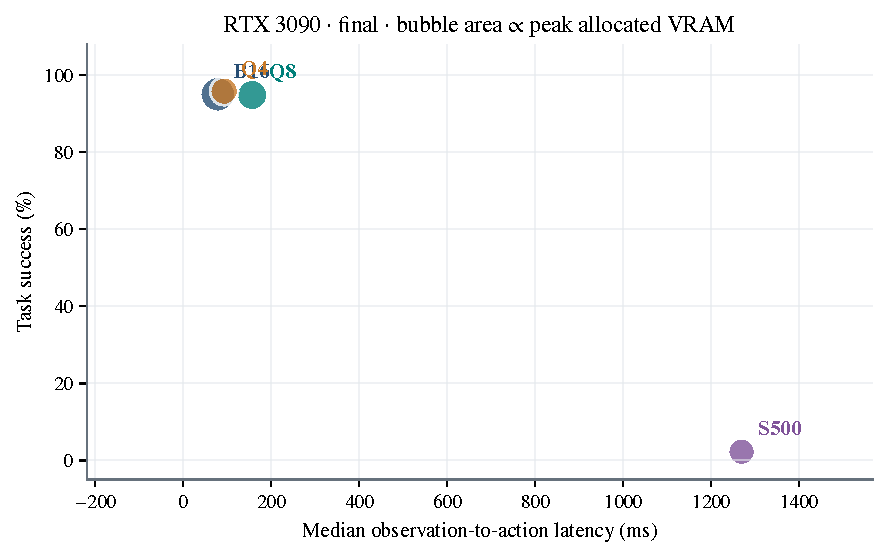
\includegraphics[width=\linewidth]{figures/F3_tradeoff.pdf}\caption{Measured success--latency trade-off. Marker area represents peak allocated GPU memory.}\end{figure}
\begin{figure}[ht]\centering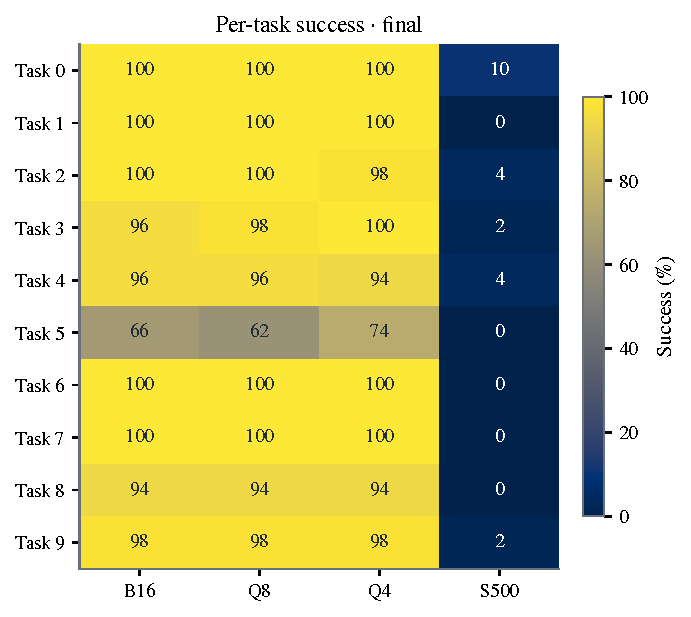
\includegraphics[width=\linewidth]{figures/F4_tasks.pdf}\caption{Task-level manipulation success; task numbers follow the committed initial-state manifest.}\end{figure}
\begin{figure}[ht]\centering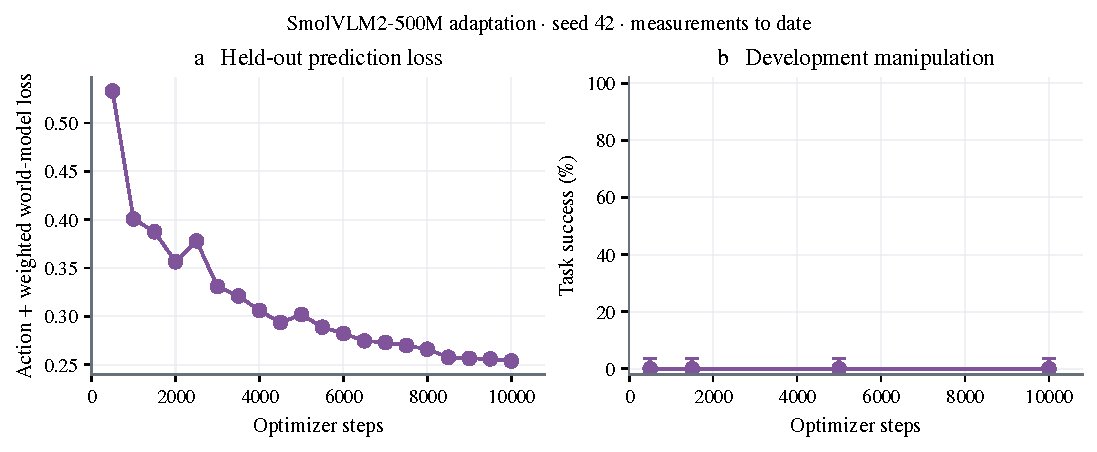
\includegraphics[width=\linewidth]{figures/F5_adaptation.pdf}\caption{Adaptation measurements from the continuing training run. Missing development rollouts are marked explicitly; prediction loss is not robot success.}\end{figure}

\FloatBarrier\section{Optional architecture confirmation}
The optional discovery study selected candidate n0008, which adds a trainable residual adapter near the end of the frozen SmolVLM decoder. A separate confirmation continued its native 5,000-step checkpoint to 10,000 steps on an RTX 5090, preserving the optimizer, seed, trajectory split, normalization and training objectives. The action head, latent predictor and conditioning adapters train; the SmolVLM and V-JEPA encoders remain frozen. This continuation is distinct from S500 in T1.

Held-out loss decreased from 0.3056 at 5,500 steps to 0.2653 at 10,000 steps (200 fixed samples). Closed-loop development evaluation completed ten valid trials, one per task, with zero successes. This small diagnostic does not establish a final success rate or performance retention; lower prediction loss did not yield successful manipulation.

Full-pipeline median/p95 latency was 302.8/407.7 ms; policy-native latency was 257.6/311.1 ms. Peak allocated inference memory was 2.97 GiB. Each mode used 500 predictions across three repetitions. Policy-native timing includes backbone preprocessing and is not neural-only timing. These RTX 5090 measurements cannot isolate a pipeline or architecture speedup against the earlier RTX 3090/PIL measurements.

The full resumable checkpoint was hash-verified before rental deletion. The matched SmolVLM baseline confirmation, full development/final trials, and fixed-checkpoint cross-hardware comparisons remain pending. Training exposure and backbone trainability differ substantially from the original paper; this experiment does not isolate undertraining, representation mismatch or a control-pipeline issue.
A subsequent processor audit identified a concrete input defect in this frozen GPU pipeline: structured image-device arguments suppressed the flat no-rescale argument. Unit-range images were scaled again, reducing pixel contrast by a factor of 255. The original results remain attributable to that pipeline; they cannot establish a limitation of SmolVLM capacity. The current plugin is corrected and a real-processor pixel-range regression passes. Corrected-input training and control evaluation are a separate recovery study; no successful recovered policy is claimed here.
\begin{figure}[ht]\centering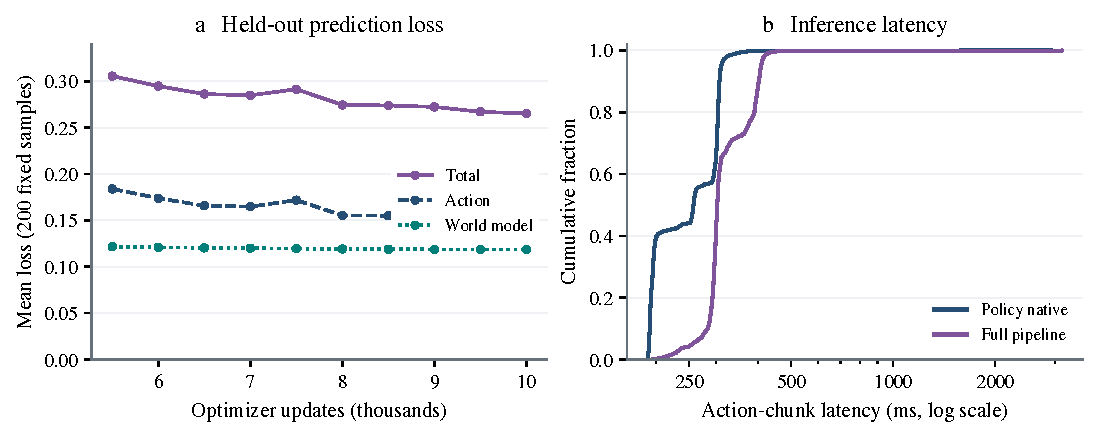
\includegraphics[width=\linewidth]{figures/F6_cloud.pdf}\caption{Separate n0008 confirmation: held-out action/world prediction loss and measured inference latency distributions on the RTX 5090. Loss points use the same 200 held-out samples; each latency curve contains 1,500 predictions. Closed-loop development success was 0/10 and is not inferred from prediction loss.}\end{figure}
\FloatBarrier\section{Corrected-input recovery}
RGB recovery adapts four final SmolVLM decoder layers from legacy 10k weights: fresh AdamW, batch eight, decoder/other rates $10^{-5}/10^{-4}$, fixed 20k cosine schedule. Data, tiling, action/world architecture and losses remain unchanged. Physical arm error on 200 held-out frames selects checkpoints; final trials are reserved.

Inference rounds nonpersistent rotary frequencies to BF16, unlike native FP32-buffer training. Changing only these buffers raises one-frame action loss 0.0460$\rightarrow$0.0618; restoring their original values reverses it exactly. Sequential local 20k tests yield 4/10 in each mode, with one gain and one loss: no aggregate control improvement.

Full-decoder/query recovery passes RTX5090 native save/resume (23.74\,GiB); isolated-loader RNG also passes a bounded four-update reproducibility check. Engineering is excluded from selection. At 2,000 query updates, held-out arm MSE is 0.0340; development yields 4/10 (diagnostic trials). A local 200-frame check preserves all 25 initial batch scores; 500 updates raise arm MSE 0.0237$\rightarrow$0.0400. Learning changes remain coupled.

At 20,000 additional updates, held-out arm RMSE was 0.153, compared with 0.283 at 500; gripper error changed from 13.6\% to 4.8\%. On two held-out frames per task, finite-draw mean arm error remains 9.9--67.2$\times$ B16 across all ten tasks.


The 20,000-update checkpoint achieved 6/10 development successes. RTX5090 inference uses 2.98\,GiB and 108.3\,ms median pipeline latency (1,500 predictions). Matched final performance retention remains untested.

\begin{figure}[ht]\centering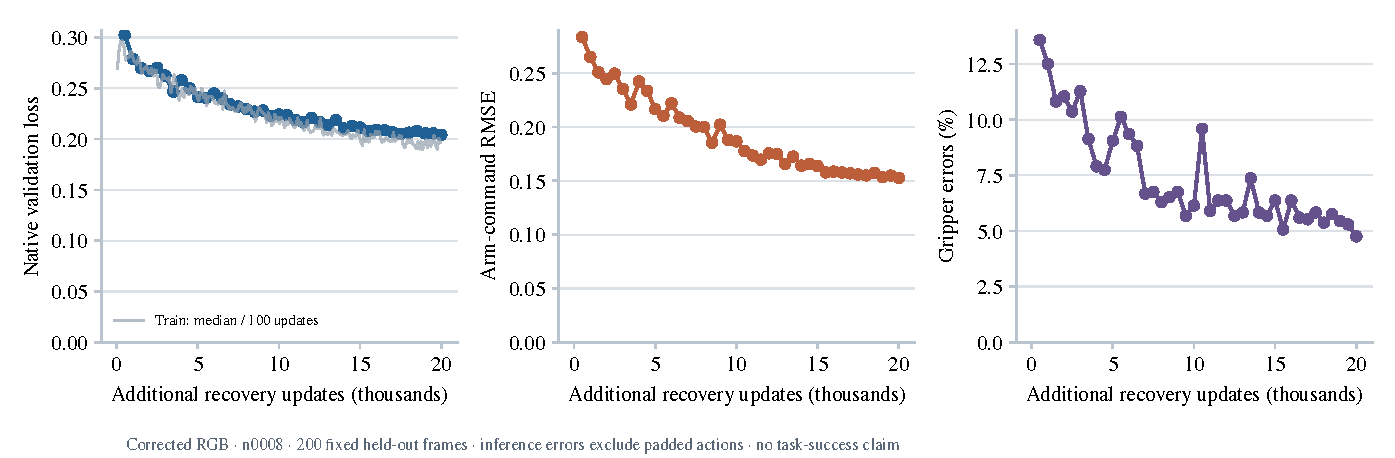
\includegraphics[width=\linewidth]{figures/F8_recovery_progress.pdf}\caption{Registered RGB-recovery validation. Physical command errors use 1,303 valid actions from the same 200 held-out frames, excluding padding. The gray curve is median training loss per 100 updates. Recovery steps are additional to the legacy 10k checkpoint. These are offline diagnostics, not LIBERO success measurements.}\end{figure}
\FloatBarrier\subsection{Expanded development comparison}
Fixed parent20k and B16 checkpoints complete 100 paired original development states on RTX3090, with identical task/state/seed membership and unchanged solver, horizon and preprocessing. B16 succeeds in 82/100 trials and SmolVLM in 31/100. Both succeed in 31 states; B16 alone succeeds in 51, SmolVLM alone in 0, and both fail in 18. These development trials include earlier diagnostic states and are not pooled with them. Different training histories and model-specific numerical loaders prevent architecture-only causal attribution. Final acceptance remains untested.

\begin{figure}[ht]\centering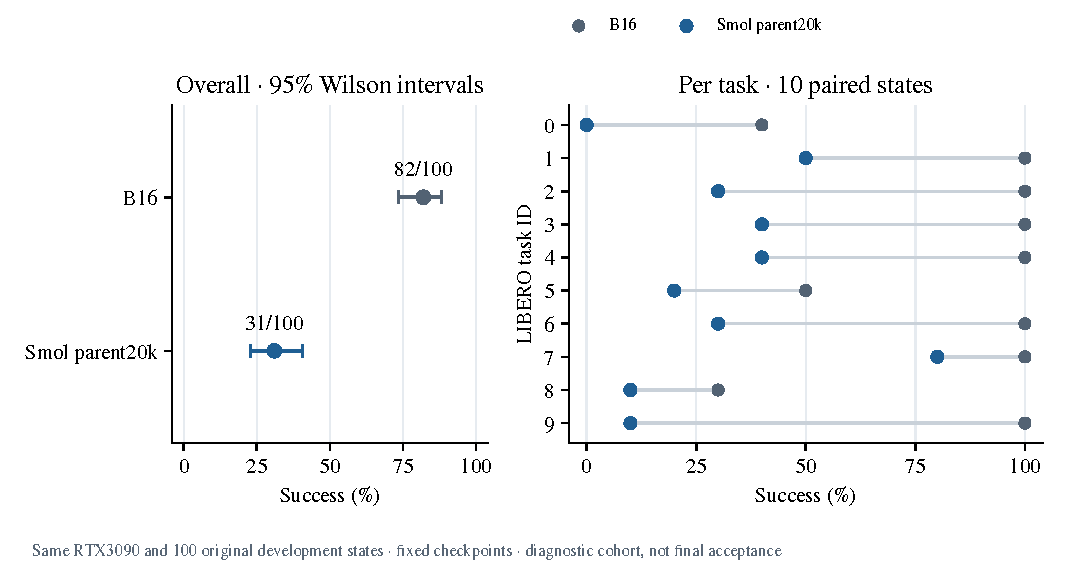
\includegraphics[width=\linewidth]{figures/F16_expanded_development.pdf}\caption{Registered expanded development comparison. Left: trial-count Wilson 95\% intervals; right: ten paired states per task. Development findings do not establish performance on the reserved official final cohort.}\end{figure}

\FloatBarrier
\section{Decision rule and limitations}
The prespecified engineering target is at least 25\% lower peak inference memory with at most a five-percentage-point success drop from B16. Estimates are reported with uncertainty; an inconclusive interval does not establish performance preservation. Retaining the world model consistently prevents module removal from masquerading as a quantization benefit. A single GPU, limited adaptation budget, and differing pretraining histories limit broader conclusions.

The inherited world-model loss uses bidirectional video embeddings; it does not measure causal future prediction. Deployment receives current observations only. Validation trajectories are held out from this adaptation, not necessarily from published models' earlier training. Checkpoint loading audits all mismatches; documented unused tensors and verified tied aliases are excluded.

Backbones retain their native processors: SmolVLM expands each 224-pixel image into seventeen 512-pixel tiles. This workload differs from Qwen's; parameter count alone does not predict latency. Neural-only timing excludes preprocessing. Input scaling and inference-buffer precision require independent checks.

\textbf{Summary.} Deployment savings and retained manipulation success must both be demonstrated.

\begin{thebibliography}{6}\small
\bibitem{vla} Sun et al. VLA-JEPA: Enhancing Vision-Language-Action Model with Latent World Model. arXiv:2602.10098, 2026.
\bibitem{libero} Liu et al. LIBERO: Benchmarking Knowledge Transfer for Lifelong Robot Learning. arXiv:2306.03310, 2023.
\bibitem{smol} Marafioti et al. SmolVLM: Redefining Small and Efficient Multimodal Models. arXiv:2504.05299, 2025.
\bibitem{jepa} Assran et al. V-JEPA 2: Self-Supervised Video Models Enable Understanding, Prediction and Planning. arXiv:2506.09985, 2025.
\bibitem{int8} Dettmers et al. LLM.int8(): 8-bit Matrix Multiplication for Transformers at Scale. \href{https://arxiv.org/abs/2208.07339}{arXiv:2208.07339}, 2022.
\bibitem{nf4} Dettmers et al. QLoRA: Efficient Finetuning of Quantized LLMs. \href{https://arxiv.org/abs/2305.14314}{arXiv:2305.14314}, 2023.
\end{thebibliography}
\end{document}
